\documentclass[12pt]{article}
%\usepackage[utf8]{inputenc}
%\documentclass[UTF8]{ctexart}
%\usepackage[UTF8, heading = false, scheme = plain]{ctex}
\usepackage{geometry}
%geometry{a4paper,scale=0.9}
\geometry{a4paper,left=1cm,right=1cm,top=1cm,bottom=2cm}
\usepackage{amsfonts}
\usepackage{color}
\usepackage{url}
%\usepackage{biblatex}
\usepackage{amsmath}
\usepackage{amssymb}
\usepackage{latexsym}
\usepackage{cite}
%\addbibresource{ref.bib}
%\bibliography{ref.bib}
\usepackage{caption}
\usepackage{graphicx, subfig}
\usepackage{float}
%\usepackage[fontset=ubuntu]{ctex}
%\usepackage{fontspec}
\usepackage{xeCJK}
%\usepackage[colorlinks,
%anchorcolor=black,
%citecolor=black]{hyperref}
%\setmainfont{SimSun}
\usepackage[section]{placeins}
\usepackage{enumitem}
\usepackage{framed}
\usepackage[framemethod=TikZ]{mdframed}
\usepackage{indentfirst}
\usepackage{setspace}%使用间距宏包
\linespread{1.5}
%\title{预备知识}
%\author{leolinuxer }
%\date{June 2020}

\title{共轭梯度法(Conjugate Gradient Method)\cite{Conjugate_Gradient_Method_No_Pain}}
\author{leolinuxer}
%\date{June 2020}

\begin{document}
%\setlength{\parindent}{0pt}
\maketitle
\tableofcontents
\section{背景和前置知识}
\subsection{CG 的适用场景}
CG(Conjugate Gradient,共轭梯度)算法是迭代式的算法,适用于求解如下形式的大规模线性方程组:
$$
Ax = b
$$
其中 $x$ 是未知向量,$b$是已知向量,$A$是已知的、对称的、正定的(或非正定)、方阵。

类似 CG 类的迭代式方法,适用于$A$是稀疏矩阵的情况。

上式的展开形式为:
$$
\begin{bmatrix}
A_{11} & A_{12} & \cdots & A_{1n} \\
A_{21} & A_{22} & \cdots & A_{2n} \\
\vdots & \vdots & \ddots & \vdots \\
A_{n1} & A_{n2} & \cdots & A_{nn} \\
\end{bmatrix}
\begin{bmatrix}
x_1 \\ x_2 \\ \vdots \\ x_n
\end{bmatrix} = 
\begin{bmatrix}
b_1 \\ b_2 \\ \vdots \\ b_n
\end{bmatrix}
$$

\subsection{内积}
两个向量 $x, y$ 的内积记作:$x^Ty$,表示对应元素的乘积和:$\sum_{i=1}^nx_iy_i$。

向量的内积满足:
$$
x^Ty = y^Tx
$$

如果 $x$ 和 $y$ 正交,则 $x^Ty = 0$。

\subsection{正定矩阵}
如果对于任意非零向量 $x$,都有:
$$
x^TAx \ge 0
$$
则称$A$为正定矩阵。

\subsection{矩阵的性质}
$$
(AB)^T = B^TA^T
$$
$$
(AB)^{-1} = B^{-1}A^{-1}
$$

\section{特征值和特征向量}
\subsection{特征向量的性质}
给定矩阵 $B$ 的特征向量 $v$,二者的乘积 $Bv$ 只会对 $v$ 形成比例变化(或反向比例变化),而不会形成旋转变化,也就是说 $Bv$ 满足: $Bv = \lambda v$,其中 $\lambda$ 是特征值。

对于任意常量 $\alpha$,向量 $\alpha v$ 也是 $B$ 的特征向量,特征值同样为 $\lambda$。这是因为 $B(\alpha v) = \alpha Bv = \lambda (\alpha v)$。

为什么需要回忆特征向量的知识点呢,这是因为迭代的方法通常都涉及到进行反复的矩阵-向量运算。当矩阵 $B$ 反复作用于特征向量 $v$ 后,会发生如下情况:
\begin{itemize}
\setlength{\itemsep}{0pt}
\setlength{\parsep}{0pt}
\setlength{\parskip}{0pt}
    \item 如果 $|\lambda| < 1$,那么 $B^i v = \lambda^i v$,当 $i$ 趋近于无穷大时,$B^i v$ 会逐渐趋于0(如图9所示);
    \item 如果 $|\lambda| > 1$,那么 $B^i v = \lambda^i v$,当 $i$ 趋近于无穷大时,$B^i v$ 会逐渐趋于无穷大(如图10所示);
\end{itemize}
\begin{figure}[H]
    \centering
    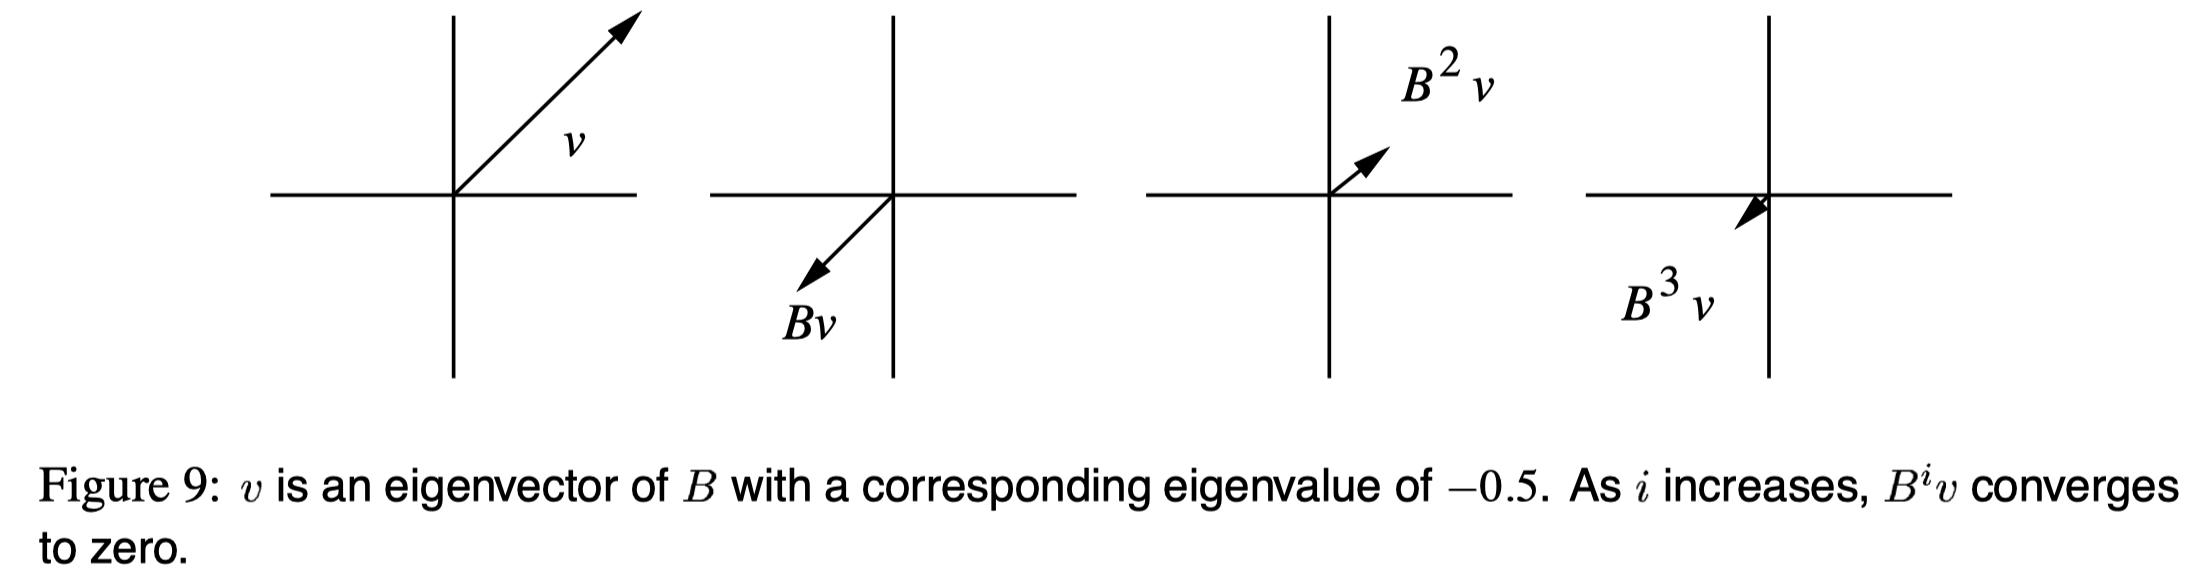
\includegraphics[width=1\textwidth]{fig/CG_Plot_Eightvalue_1.png}
\end{figure}
\begin{figure}[H]
    \centering
    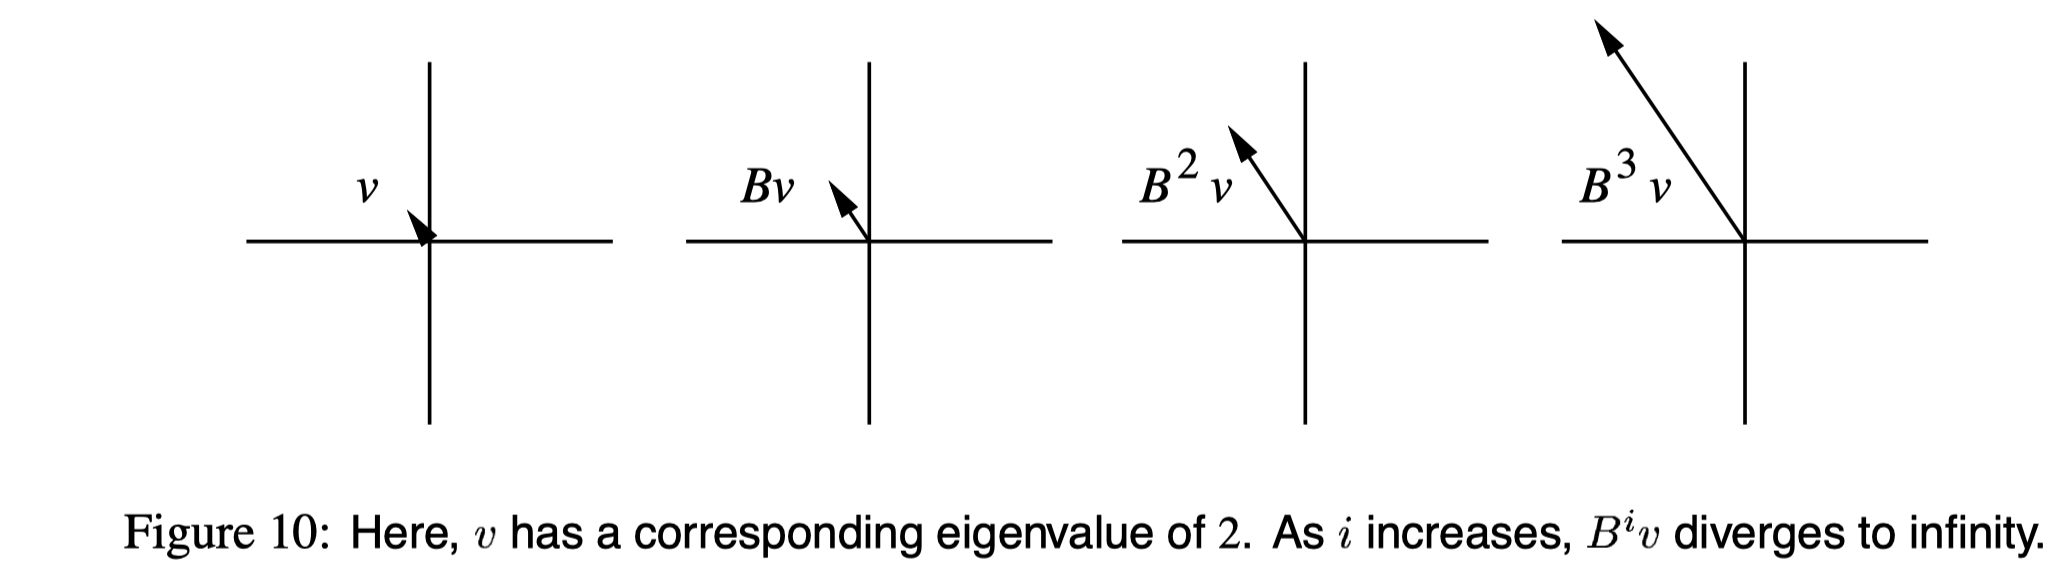
\includegraphics[width=1\textwidth]{fig/CG_Plot_Eightvalue_2.png}
\end{figure}

\textbf{如果 $B$ 是对称矩阵,那么 $B$ 存在 $n$ 个线性无关的特征向量 $v_1, v_2, \cdots, v_n$}(注意不是唯一集合,因为特征向量可以进行比例变换)和对应的 $n$ 个特征值 $\lambda_1, \lambda_2, \cdots, \lambda_n$(特征值是唯一的,特征值间可以相等,也可以不等)。
 
\subsection{谱半径}
因为对称矩阵 $B$ 的 $n$ 个特征向量是线性无关的,所以\textbf{这组特征向量构成了空间 $\mathbb{R}^n$ 的一组正交基}。所以,当 $B$ 与非特征向量 $x$ 进行乘法时,可以把 $x$ 用它的特征向量进行表示,然后分别观察在各个基上结果的变化。如图11所示,给定向量 $x$,将其表示为两个基向量 $v_1, v_2$ 的和。那么 $Bx = B(v_1 + v_2) = Bv_1 + Bv_2$,所以 $B^ix = B^iv_1 + B^iv_2 = \lambda^i_1 v_1 + \lambda^i_2 v_2$。如果所有的特征值都小于1,那么 $B^ix$会趋近于0;如果至少有一个特征值大于1,那么 $B^ix$ 会趋近于无穷大。由此引出了矩阵的 \textbf{谱半径(spectral radius)}:
 $$
 \rho (B) = \max|\lambda_i|, \qquad \lambda_i\text{是} B \text{的特征向量}
 $$
 
 如果期望 $B^ix$ 迅速趋近于0,那么 $rho(B) < 1$,并且越小越好。
 \begin{figure}[H]
    \centering
    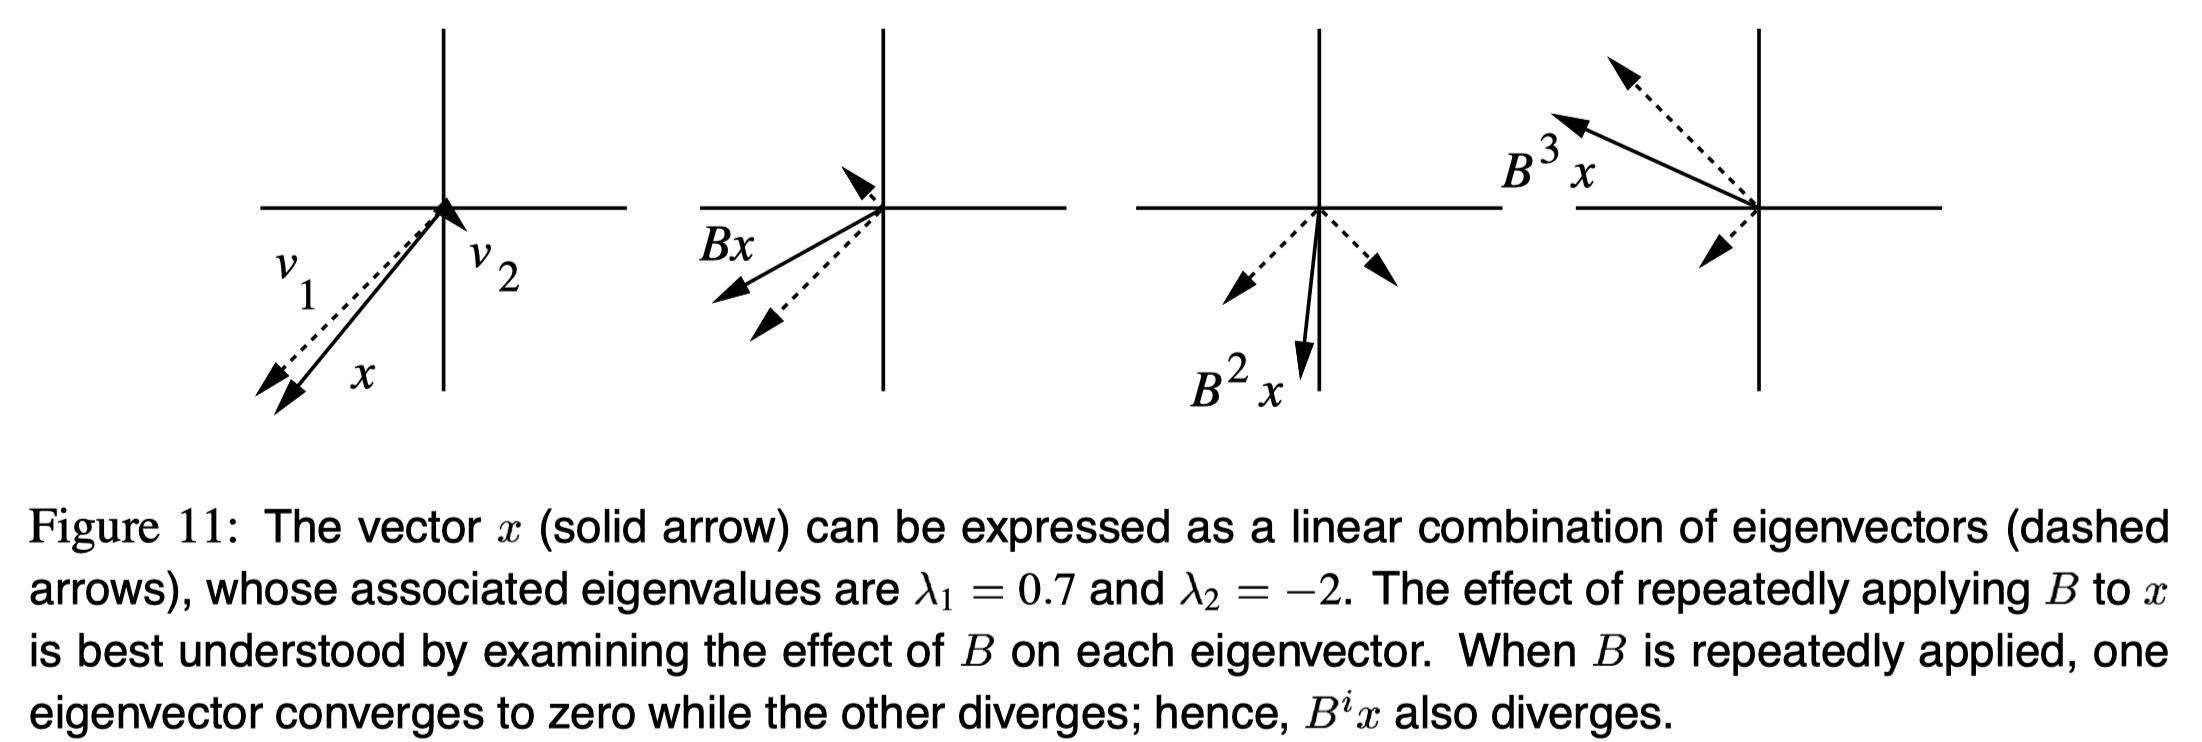
\includegraphics[width=1\textwidth]{fig/CG_Plot_Eightvalue_3.png}
\end{figure}

 \subsection{正定矩阵的特征值}
 \textbf{正定矩阵的特征值均大于0},证明如下
\begin{align*}
Bv &= \lambda v \\
v^T B v &= \lambda v^T v
\end{align*}

因为 $B$ 是正定矩阵,所以对于任意非零向量 $v$ 都有 $v^T B v > 0$,所以必有 $\lambda > 0$。
 
\subsection{一个具体的例子}
给定矩阵 $A$,它的特征向量 $v$ 和特征值 $\lambda$ 满足:
$$
Av = \lambda v = \lambda Iv \Rightarrow (\lambda I - A) v = 0
$$

因为 $v$ 是非零向量,所以 det($\lambda I - A) = 0$,以后文会用到的 $A = \begin{bmatrix}3 & 2 \\ 2 & 6\end{bmatrix}$ 为例,有:
$$
\text{det}\begin{bmatrix}
\lambda - 3 & -2 \\ -2 & \lambda -6
\end{bmatrix} = \lambda^2 - 9\lambda + 14 = (\lambda - 7)(\lambda - 2)
$$

所以,特征是是 $\lambda_1 = 7, \lambda_2 = 2$。当 $\lambda_1 = 7$ 时,有:
$$
(\lambda I - A) v = \begin{bmatrix}4 & -2 \\ -2 & 1\end{bmatrix}\begin{bmatrix}v_1 \\ v_2 \end{bmatrix} = 0
$$
$$
\therefore 4v_1 - 2v_2 = 0
$$

任意满足该方程的解都可以构成对应的特征向量,比如 $v = [1, 2]^T$。同理,可以求得特征值 $\lambda_2 = 2$ 对应的特征向量为$v = [-2, 1]^T$。如下图所示,$A$ 的两个特征向量对应了图中的两个箭头,并且较大的特征值 $\lambda_1 = 7$ 对应了更陡的斜率。

\begin{figure}[H]
    \centering
    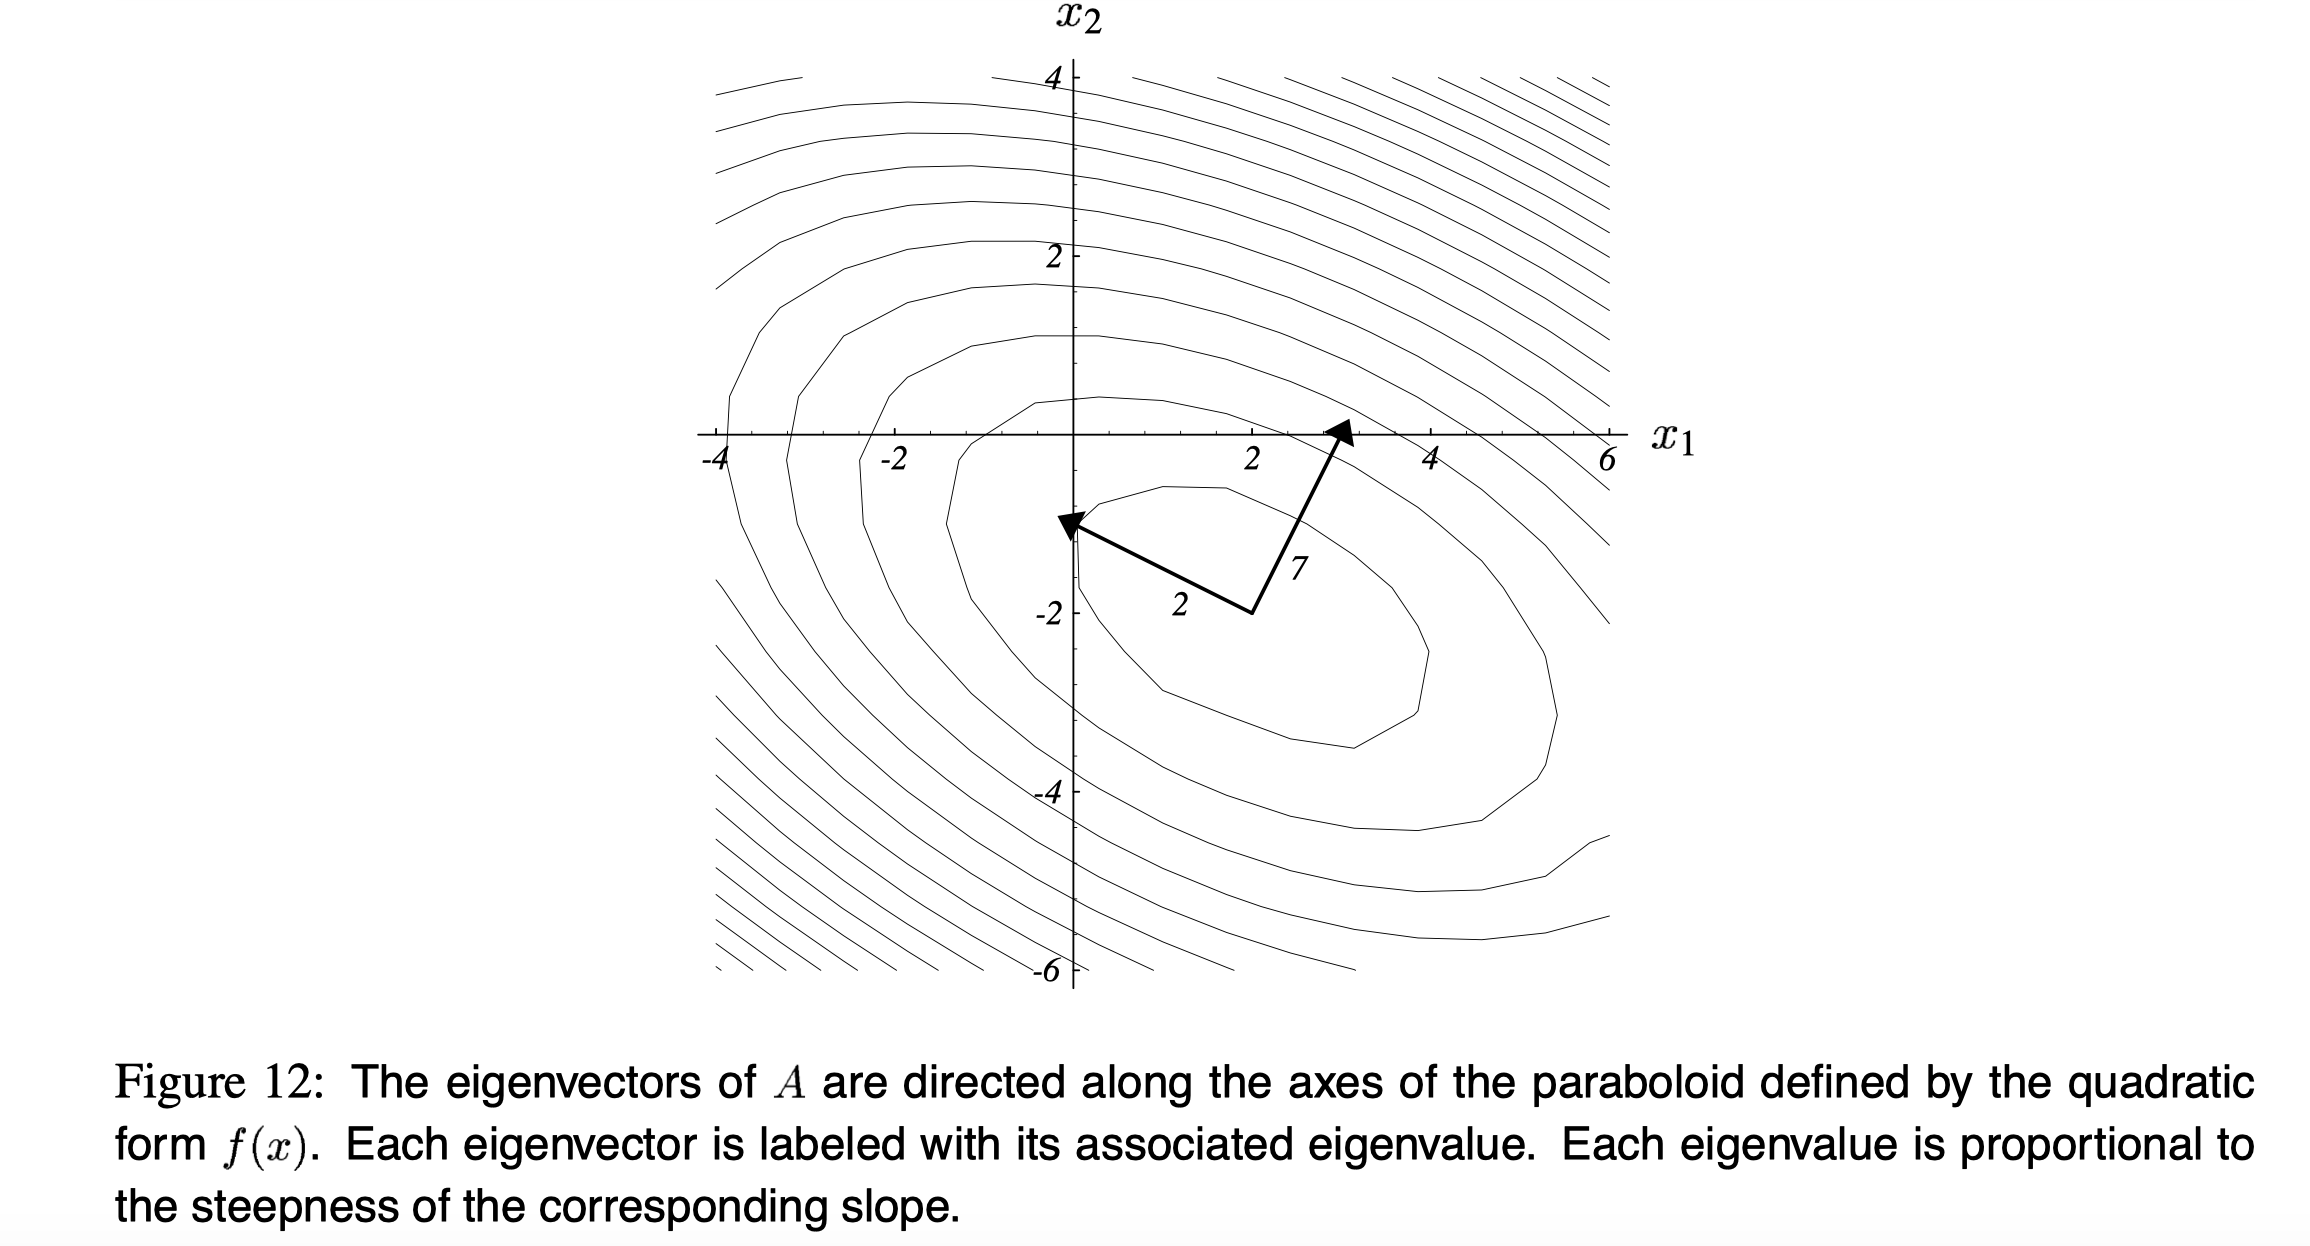
\includegraphics[width=1\textwidth]{fig/CG_Plot_Eightvalue_4.png}
\end{figure}

\section{二次型(Quadratic Form)}
向量的二次型形式为:
$$
f(x) = \frac{1}{2}x^TAx - b^Tx + c
$$
其中 $A$ 是矩阵,$b$ 和 $x$ 是向量,$c$ 是常量。

\textbf{如果 $A$ 是对称正定阵,那么 当 $Ax = b$ 时,$f(x)$ 取得最小值}。

\subsection{一个具体的例子}
$$
A = \begin{bmatrix} 3 & 2 \\ 2 & 6 \end{bmatrix} \qquad 
b = \begin{bmatrix} 2 \\ -8 \end{bmatrix} \qquad 
c = 0
$$

$Ax = b$ 的图像如下:
\begin{figure}[H]
    \centering
    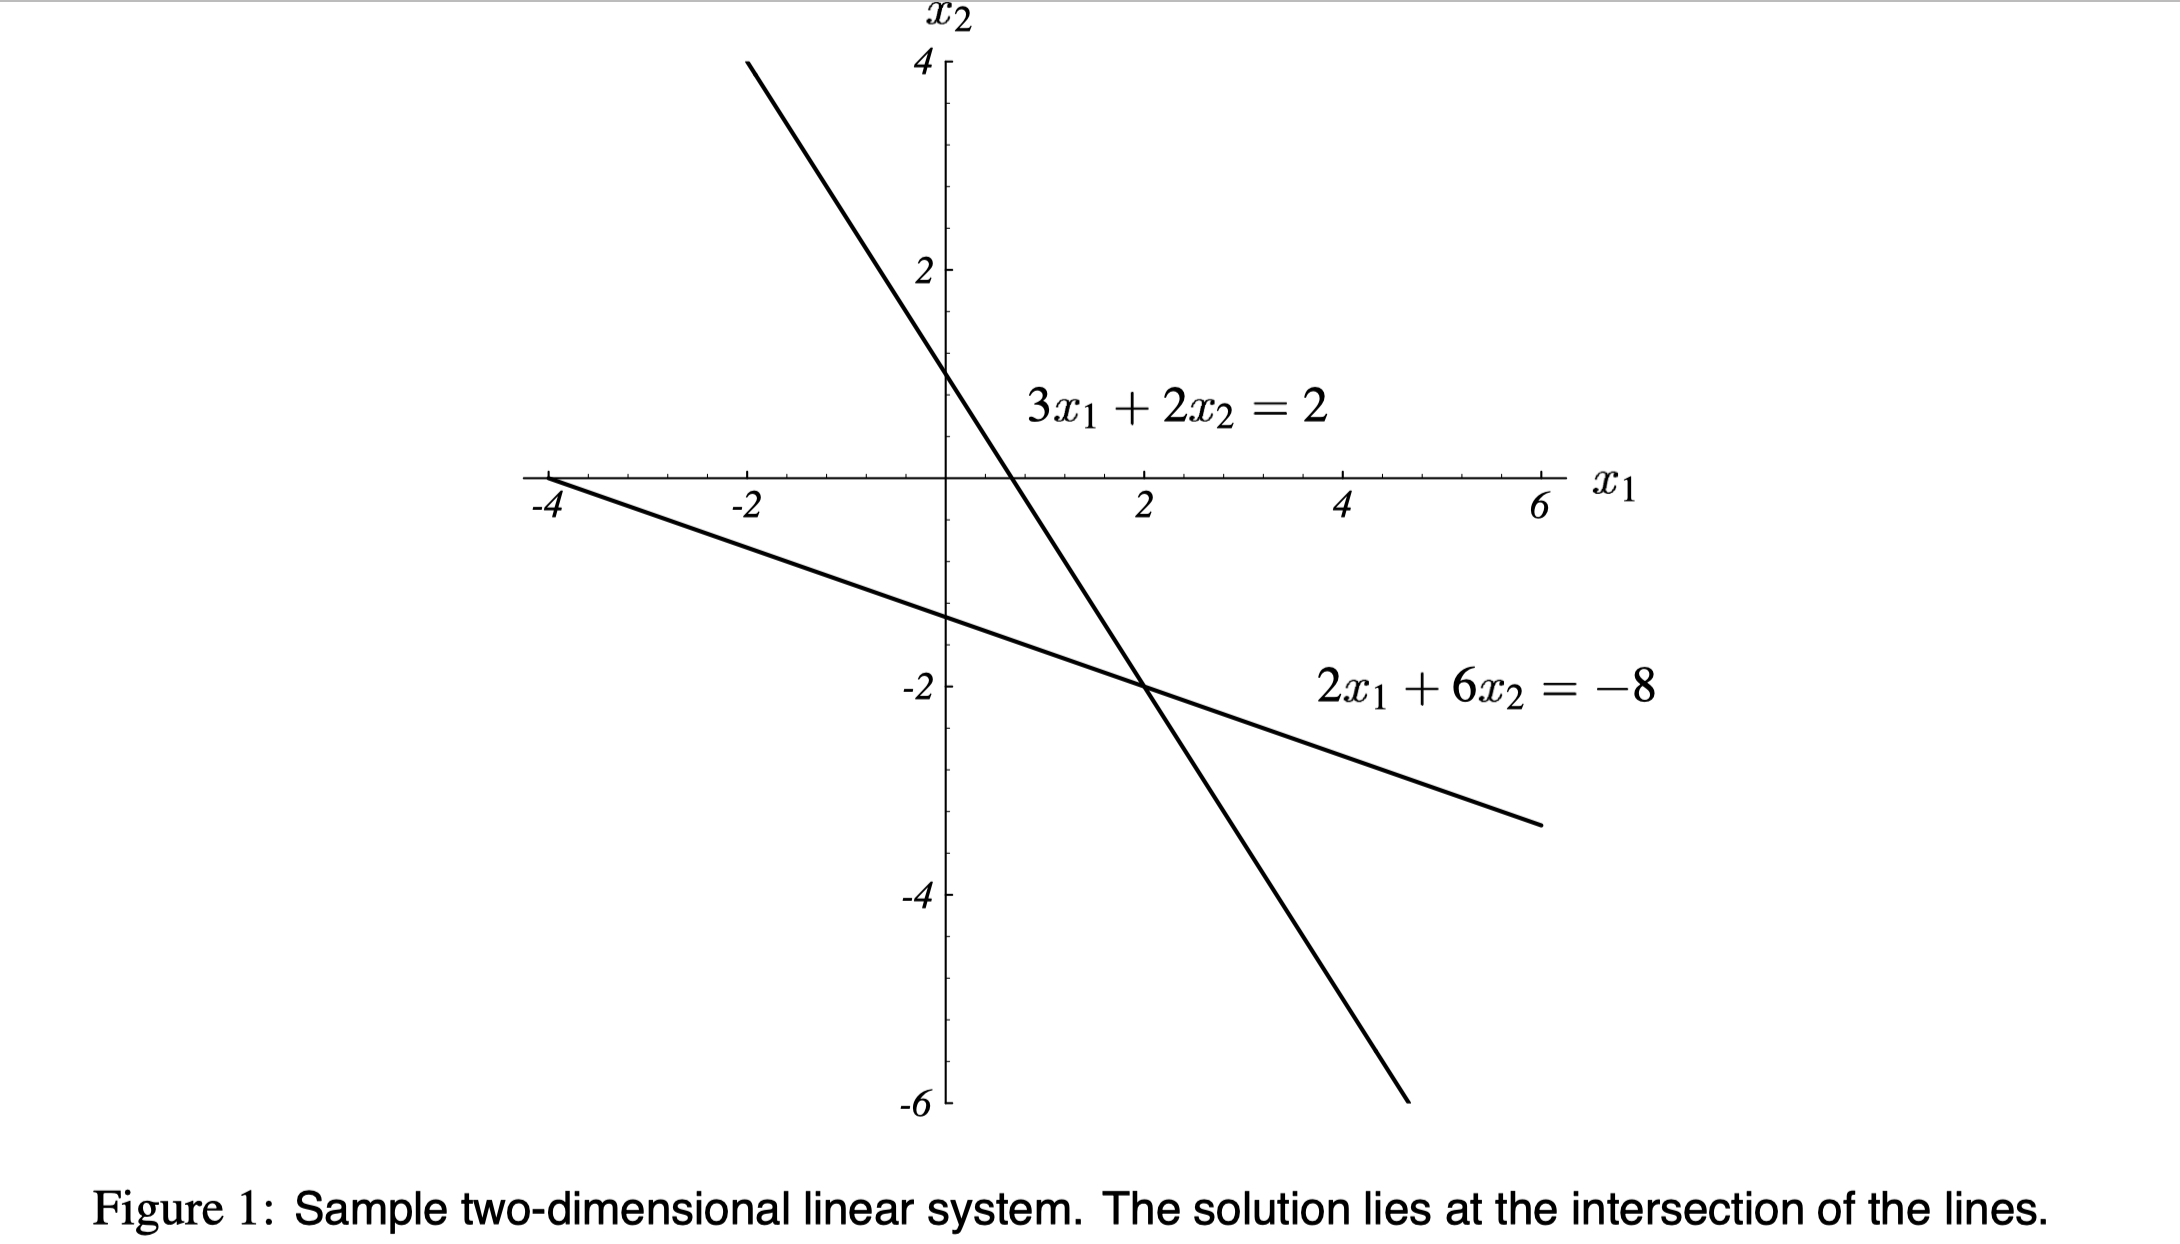
\includegraphics[width=.8\textwidth]{fig/CG_Plot_Eq_1.png}
\end{figure}
方程的解位于 $n=2$ 维超平面的交点处,每个超平面有 $n-1=1$ 维。本方程的解为 $x = [2, -2]^T$;

对应的二次型 $f(x)$ 的图像为:
\begin{figure}[H]
    \centering
    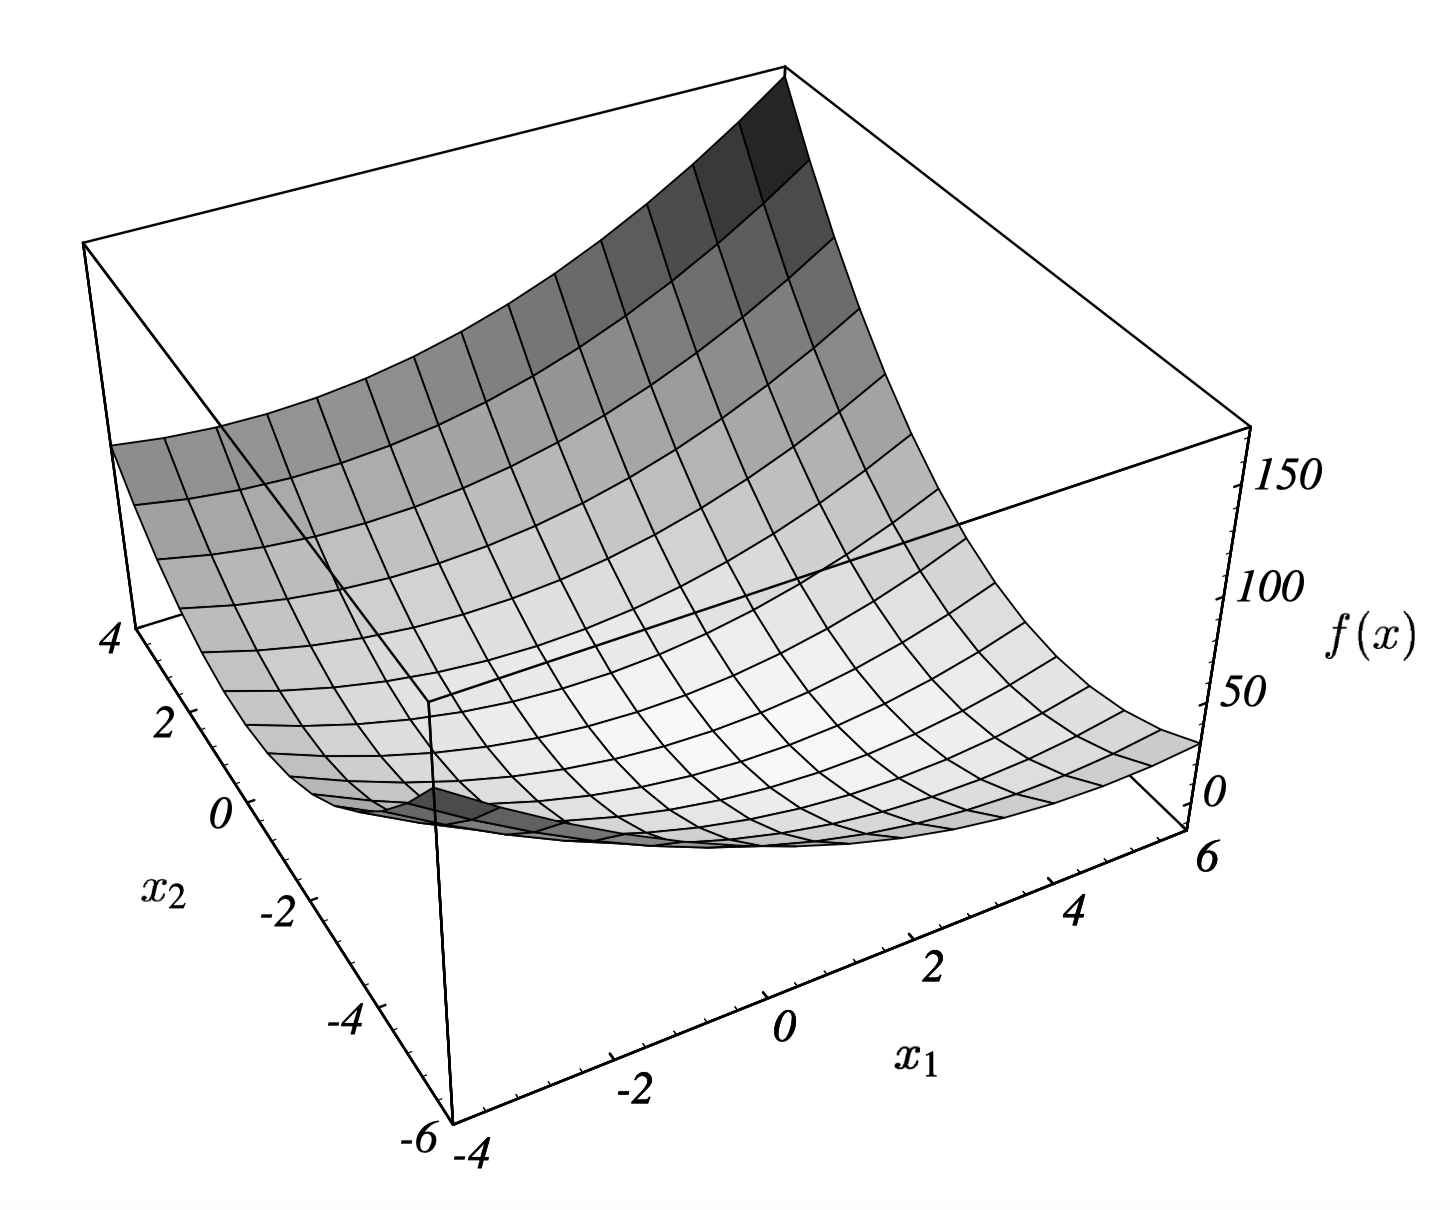
\includegraphics[width=.6\textwidth]{fig/CG_Plot_Eq_2.png}
\end{figure}

它的等高线图如下:
\begin{figure}[H]
    \centering
    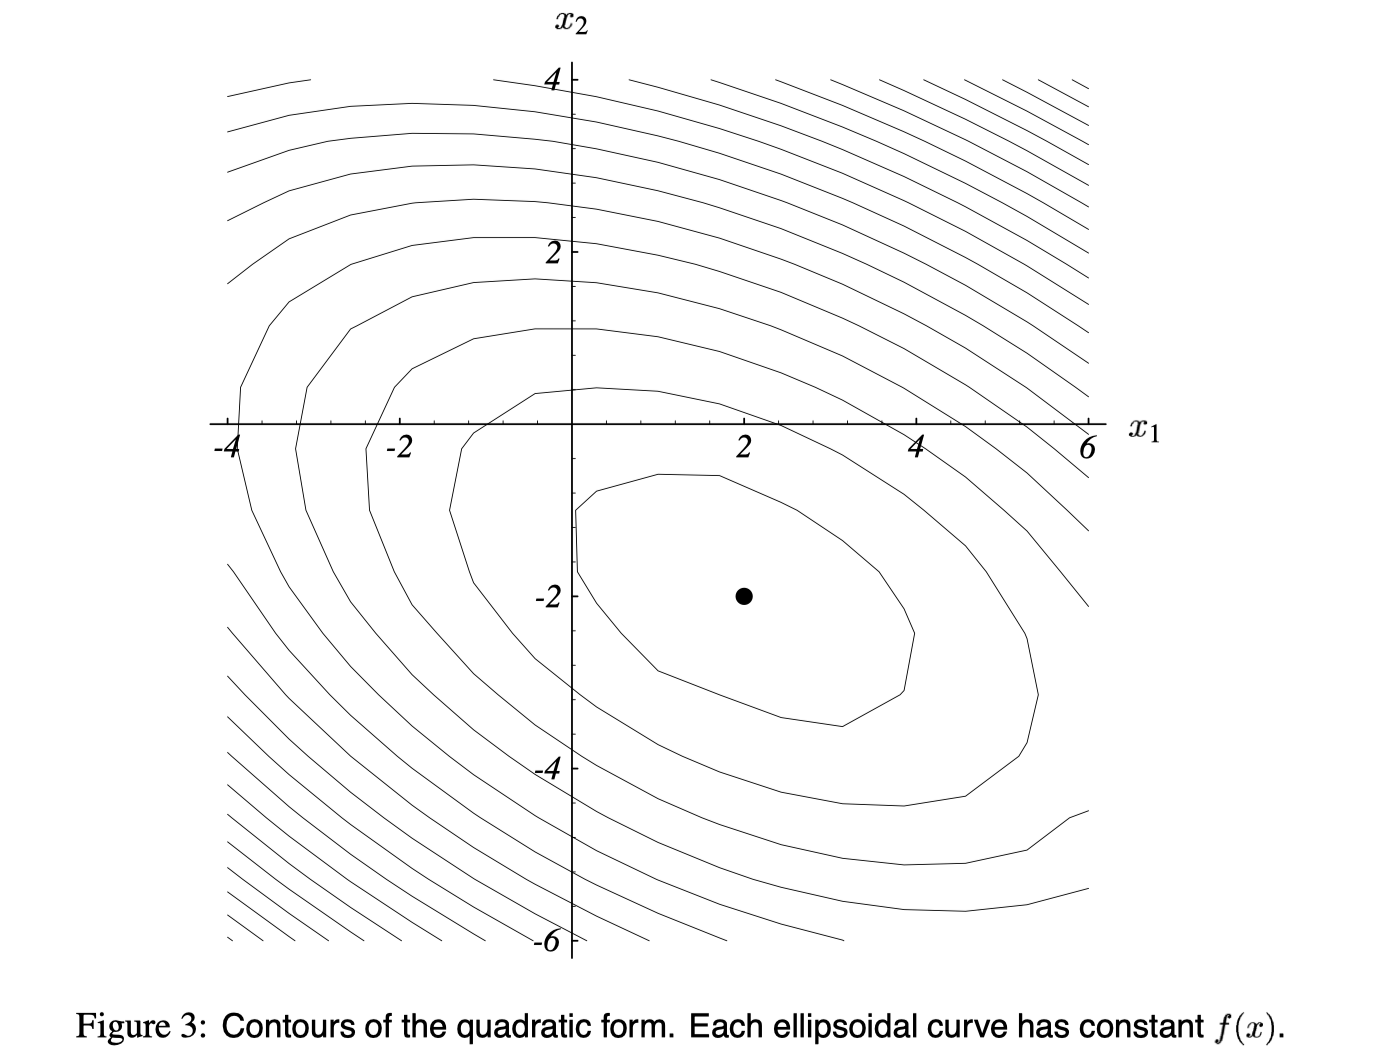
\includegraphics[width=.6\textwidth]{fig/CG_Plot_Eq_3.png}
\end{figure}

因为 $A$ 是正定矩阵,所以 $f(x)$ 的形状为抛物面形。

\subsection{梯度向量}
$f(x)$ 的梯度为:
$$
f'(x) = \begin{bmatrix}
\frac{\partial}{\partial x_1}f(x) \\
\frac{\partial}{\partial x_2}f(x) \\
\vdots \\
\frac{\partial}{\partial x_n}f(x) \\
\end{bmatrix}
$$

上面例子的梯度向量如下图所示:
\begin{figure}[H]
    \centering
    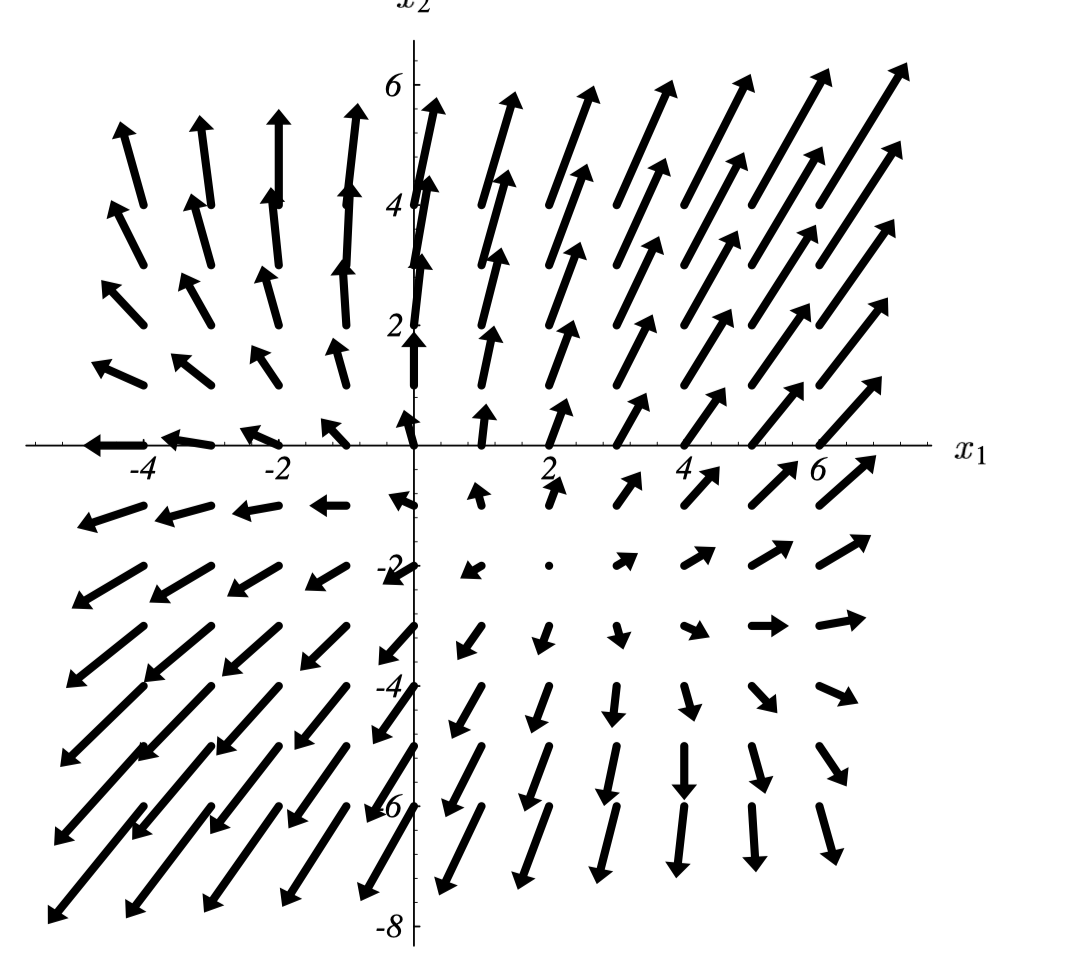
\includegraphics[width=.4\textwidth]{fig/CG_Plot_Eq_4.png}
\end{figure}
当 $f'(x) = 0$ 时,$f(x)$ 可以取得最小值。

根据$f(x) = \frac{1}{2}x^TAx - b^Tx + c$ ,有:
$$
f'(x)  = \frac{1}{2}A^Tx + \frac{1}{2}Ax + b
$$

如果 $A$ 是对称矩阵,那么有
$$
f'(x) = Ax - b
$$

所以,当 $f'(x) = Ax - b = 0$ 时,$f(x)$ 有最小值。也就是说,$Ax=b$的解是 $f(x)$ 的 critical point。如果 $A$ 是正定对称阵,那么$Ax=b$ 的解对应 $f(x)$  的最小值;

如果 $A$ 不是对称阵,那么根据$f'(x) = 0$ 有:$\frac{1}{2}(A^T+A)x = b$,并且 $\frac{1}{2}(A^T+A)$ 是对称的。

\subsection{进一步解释}
根据 $f(x) = \frac{1}{2}x^TAx - b^Tx + c$,我们可以知道如果 $A$ 是对称阵(无论是否正定),对于任意点 $p$ 和 $x = A^{-1}b$,都有:
$$
f(p) = f(x) + \frac{1}{2}(p-x)^TA(p-x)
$$

如果 $A$ 是正定的,那么根据正定矩阵的性质,对于任意$p \neq x$,都有 $\frac{1}{2}(p-x)^TA(p-x) > 0$,所以 $p = x$ 是 $f(x)$ 的最小值解。

\begin{framed}
\textbf{证明:如果 $A$ 是对称正定阵,那么 $Ax=b$ 的解最小化二次型}

假定 $A$ 是对称阵,$e$ 是误差项,那么有:
\begin{align*}
f(x+e) &= \frac{1}{2}(x+e)^TA(x+e) - b^T(x+e) + c \\
	  &= \frac{1}{2}x^TAx + e^TAx + \frac{1}{2}e^TAe - b^Tx - b^Te + c \\
	  &= \frac{1}{2}x^TAx - b^Tx + c + e^Tb + \frac{1}{2}e^TAe - b^Te \\
	  &= f(x) + \frac{1}{2}e^TAe
\end{align*}

如果 $A$ 同时也是正定的,那么对于任意 $e \neq 0$,都有 $\frac{1}{2}e^TAe > 0$;所以,$x$ 是 $f(x)$ 的最小值解。证毕。

进而,假定 $p = x + e$,即 $e = p - x$,那么有:
\begin{align*}
f(p) &= f(x + e) \\
      &= f(x) + \frac{1}{2}e^TAe \\
      &= f(x) + \frac{1}{2}(p-x)^TA(p-x)
\end{align*}
\end{framed}

不同 $A$ 的正定情况,对应着不同的图像如下:
\begin{figure}[H]
    \centering
    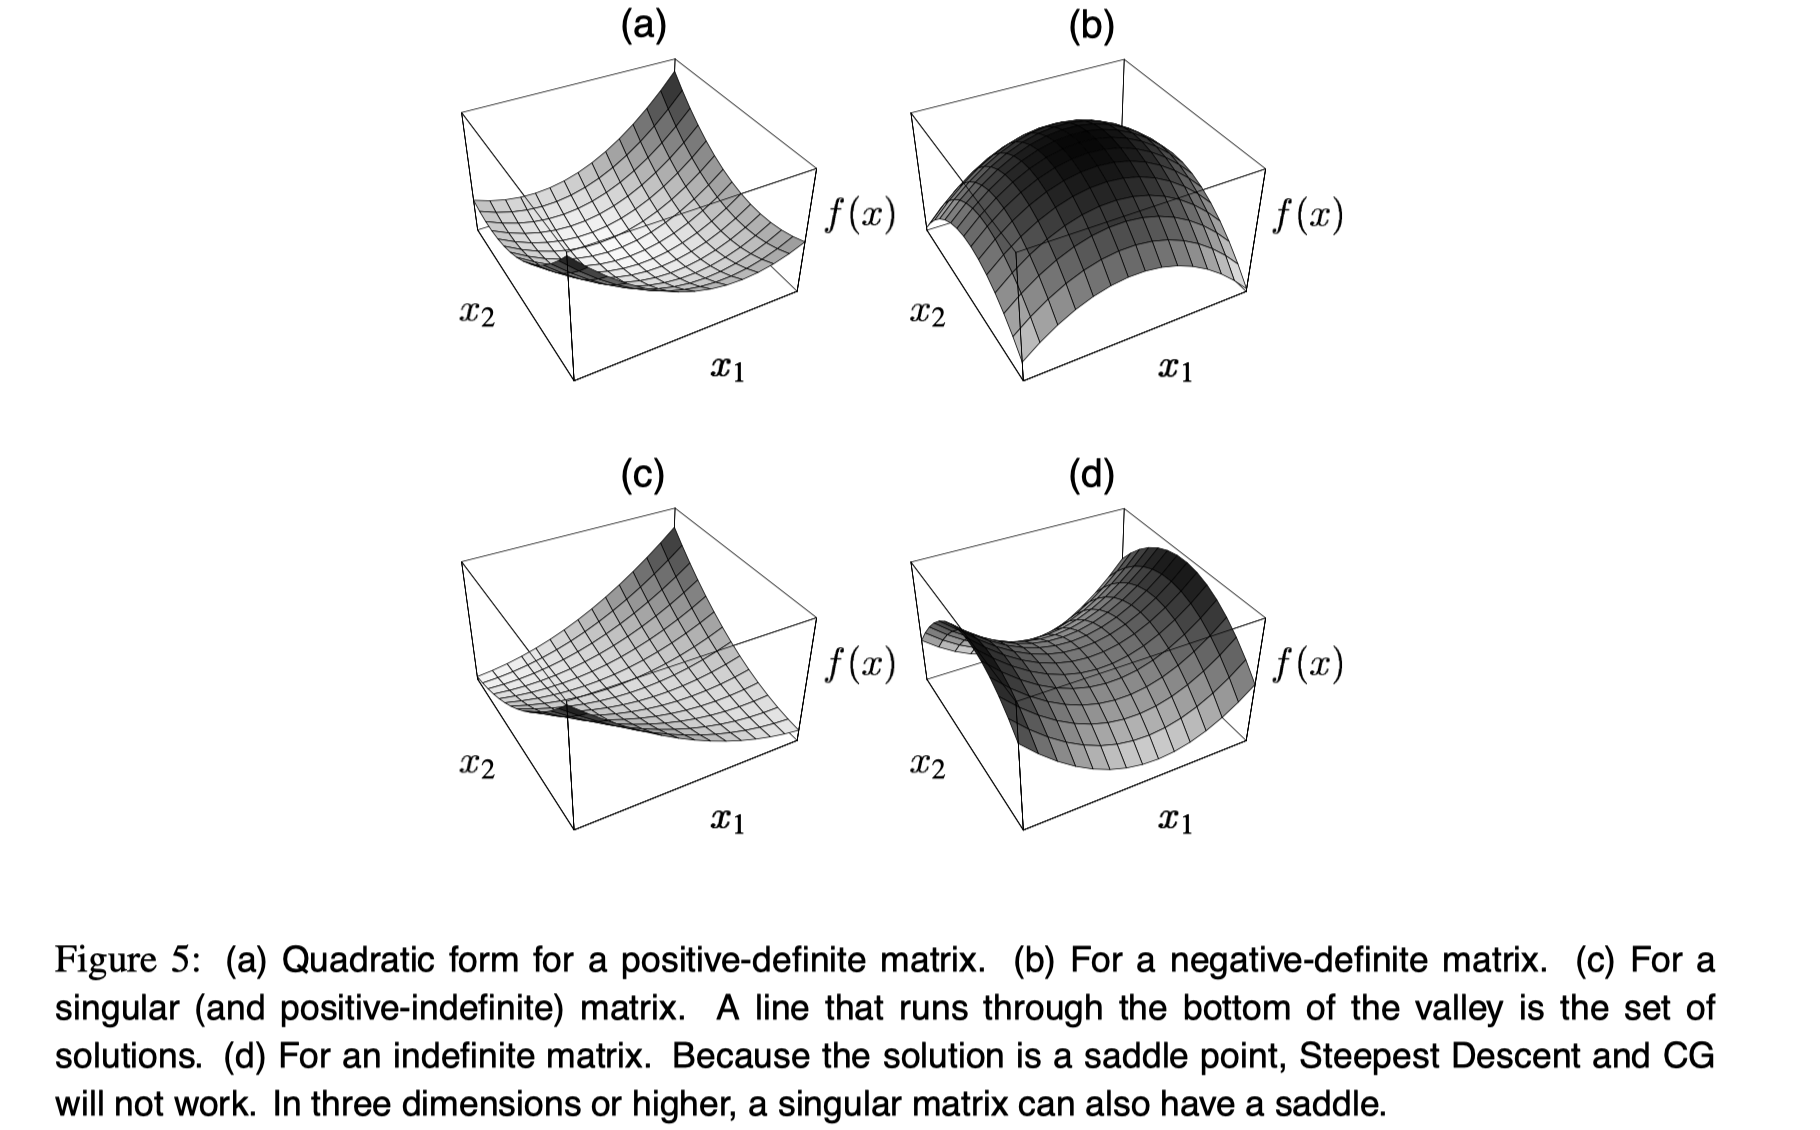
\includegraphics[width=1\textwidth]{fig/CG_Plot_Eq_5.png}
\end{figure}

\section{最速下降法(Steepest Descent)}
\subsection{最速下降法过程推导}
最速下降法:从任意点 $x_0$ 出发,沿着梯度下降,途经点为 $x_1, x_2, \cdots $ 直到足够接近解 $x$。其中,每次下降都选择 $f$ 下降最快的方向,也就是 $f'(x_i)$ 的反方向,即:$-f'(x_i) = -Ax_i + b$。

定义如下符号:
\begin{itemize}
\setlength{\itemsep}{0pt}
\setlength{\parsep}{0pt}
\setlength{\parskip}{0pt}
    \item 误差 $e_i = x_i - x$,表示 $x_i$ 与 $x$ 的接近程度;
    \item 余量$r_i = b - Ax_i$,表示 $Ax_i$ 与 $b$ 的接近程度;显然,有:$r_i = -Ae_i$,所以可以把 $r_i$ 想象为误差 $e_i$ 经过矩阵 $A$ 变换后得到的量。同时,有 $r_i = -f'(x_i)$,也就是说 $r_i$ 就是最速下降的方向。
\end{itemize}

假定从 $x_0 = [-2, -2]^T$ 出发,沿着最速下降方向(图6(a)的实现方向)前进,到达:
$$
x_1 = x_0 + \alpha r_0
$$

其中 $\alpha$ 是前进的步长,那么,应该向前走多远呢?

可以采用线搜索(line search)的方法,寻找到能够使得沿着该方向前进后,$f$ 取得最小值的最佳 $\alpha$。如图6(b)所示,垂直的平面是最速下降的方向,需要找到该平面和抛物面的交点。图6(c)是相交得到的抛物线(注意,横轴为 $\alpha$,纵轴为 $f(x_i + \alpha r_i))$;那么,该如何确定 $\alpha$ 呢,其实就是要找到该抛物线的最低点。

显然,当 $\frac{d}{d\alpha}f(x_1) = 0$ 时,能够求得 $f$ 的最小值。根据链式法则,有:$\frac{d}{d\alpha}f(x_1) = f'(x_1)^T\frac{d}{d\alpha}x_1 = f'(x_1)^Tr_0$,令该式为 0,即 $f'(x_1)^Tr_0 = 0$,也就是说,\textbf{此时 $f'(x_1)$ 与 $r_0$ 正交},如图6 (d) 所示。
\begin{figure}[H]
    \centering
    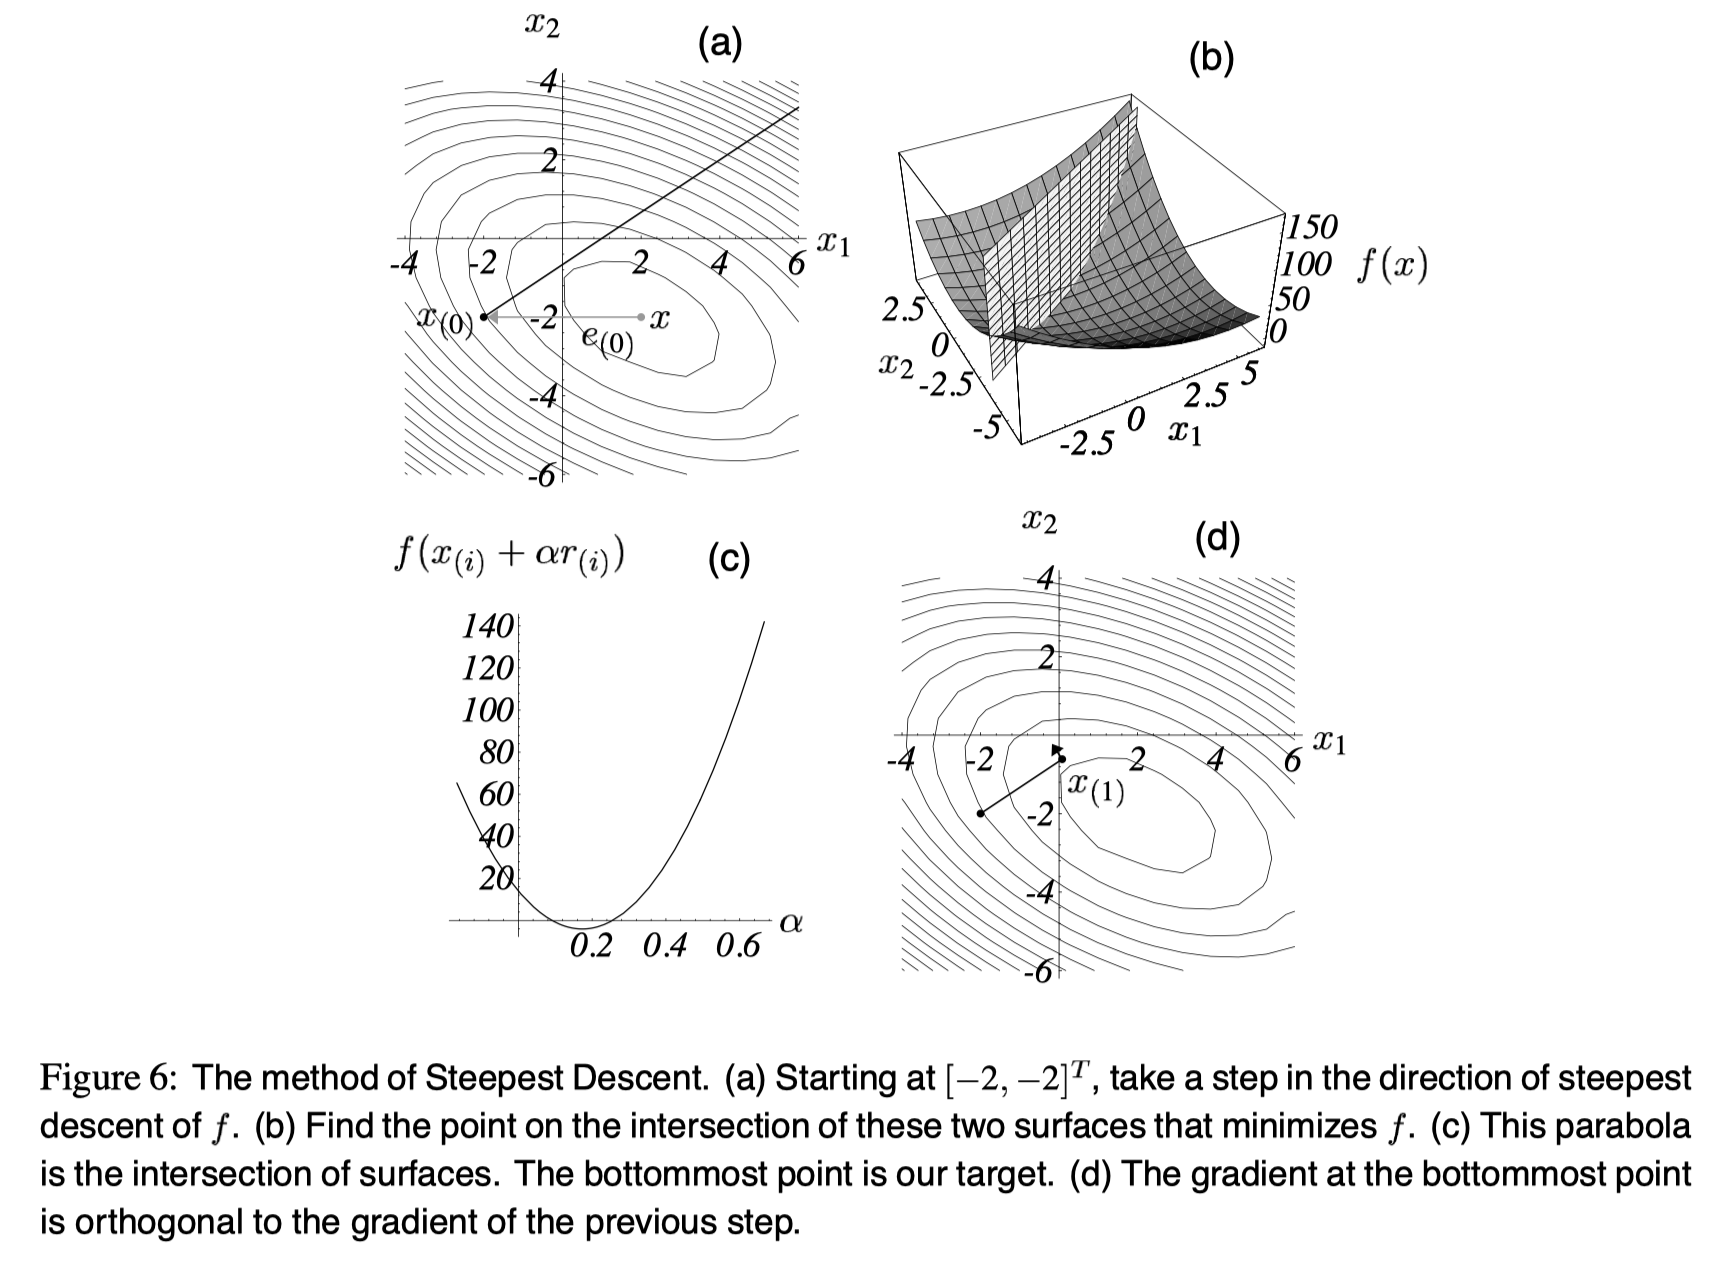
\includegraphics[width=1\textwidth]{fig/CG_Plot_SD_1.png}
\end{figure}

另外,从图7也可以看出来,为什么 $f'(x_1)$ 需要与 $r_0$ 正交。图7的实线方向是 $f'(x_1)$ 的方向(也就是 line search 的方向),该实线上不同的点有不同的梯度方向(实线箭头),对应了 $f$ 的不同的下降速率(虚线箭头),显然当下降速率为 0 时,$f$ 下降的最多,也就是说,此时的梯度与 $f'(x_1)$ 是正交的。
\begin{figure}[H]
    \centering
    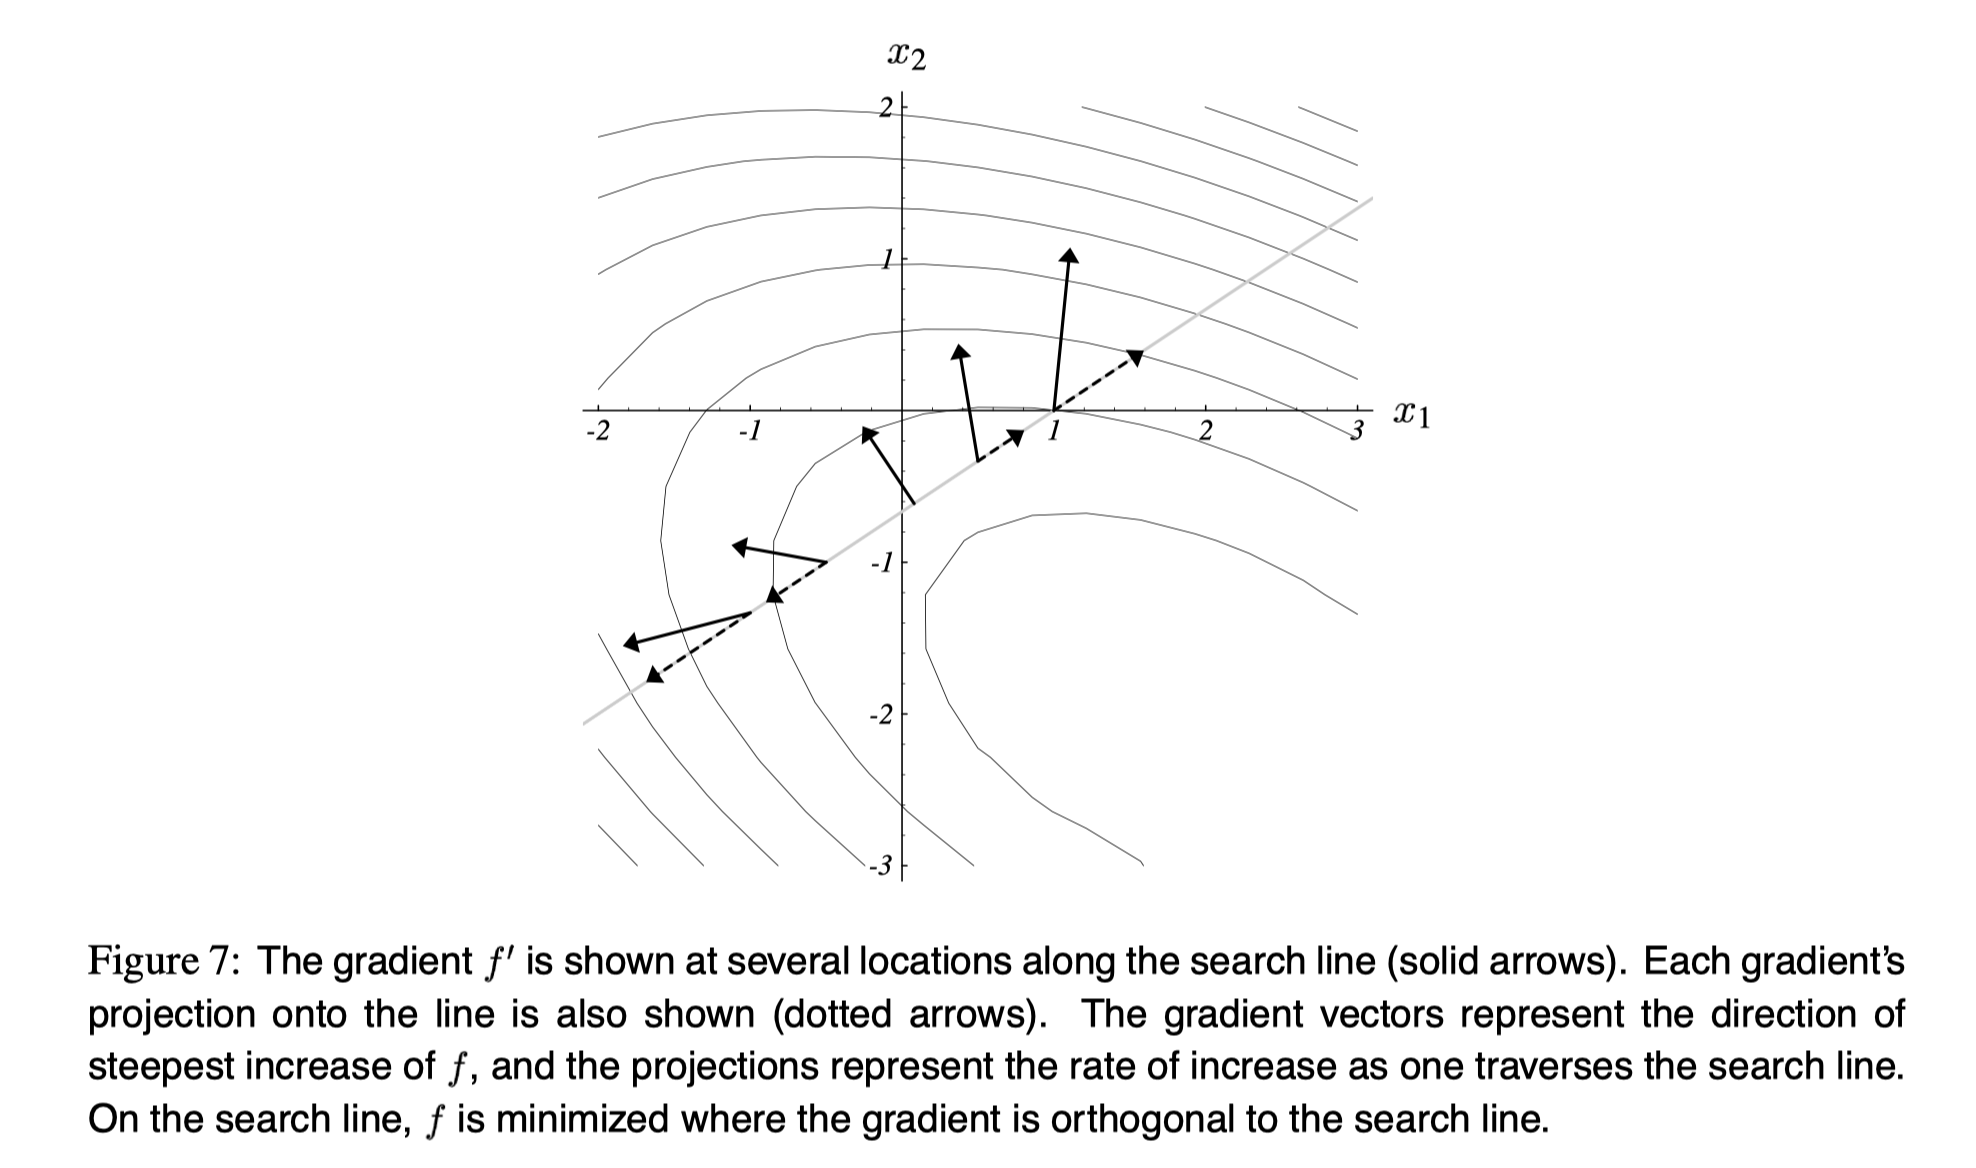
\includegraphics[width=1\textwidth]{fig/CG_Plot_SD_2.png}
\end{figure}

因为有 $f'(x_1) = -r_1$,所以可以如下推导出 $\alpha$:
\begin{align*}
f'(x_1) r_0 &= 0 \Rightarrow \\
r_1 r_0 &= 0 \Rightarrow \\
(b - Ax_1)^T r_0 &= 0 \\
(b - A(x_0 + \alpha r_0))^T r_0 &= 0 \\
(b - Ax_0)^T r_0 - \alpha (A r_0)^T r_0 &= 0 \\
(b - Ax_0)^T r_0 &=  \alpha (A r_0)^T r_0 \Rightarrow \\
r^T_0 r_0 &= \alpha r^T_0(Ar_0) \Rightarrow \\
\alpha &= \frac{r^T_0 r_0 }{r^T_0 A r_0}
\end{align*}

汇总后,就得到了最速下降法的具体过程:
$$
r_i = b - Ax_i
$$
$$
\alpha_i = \frac{r^T_0 r_0 }{r^T_0 A r_0}
$$
$$
x_{i+1} = x_i + \alpha_i r_i
$$

图8是该过程的具体示例:
\begin{figure}[H]
    \centering
    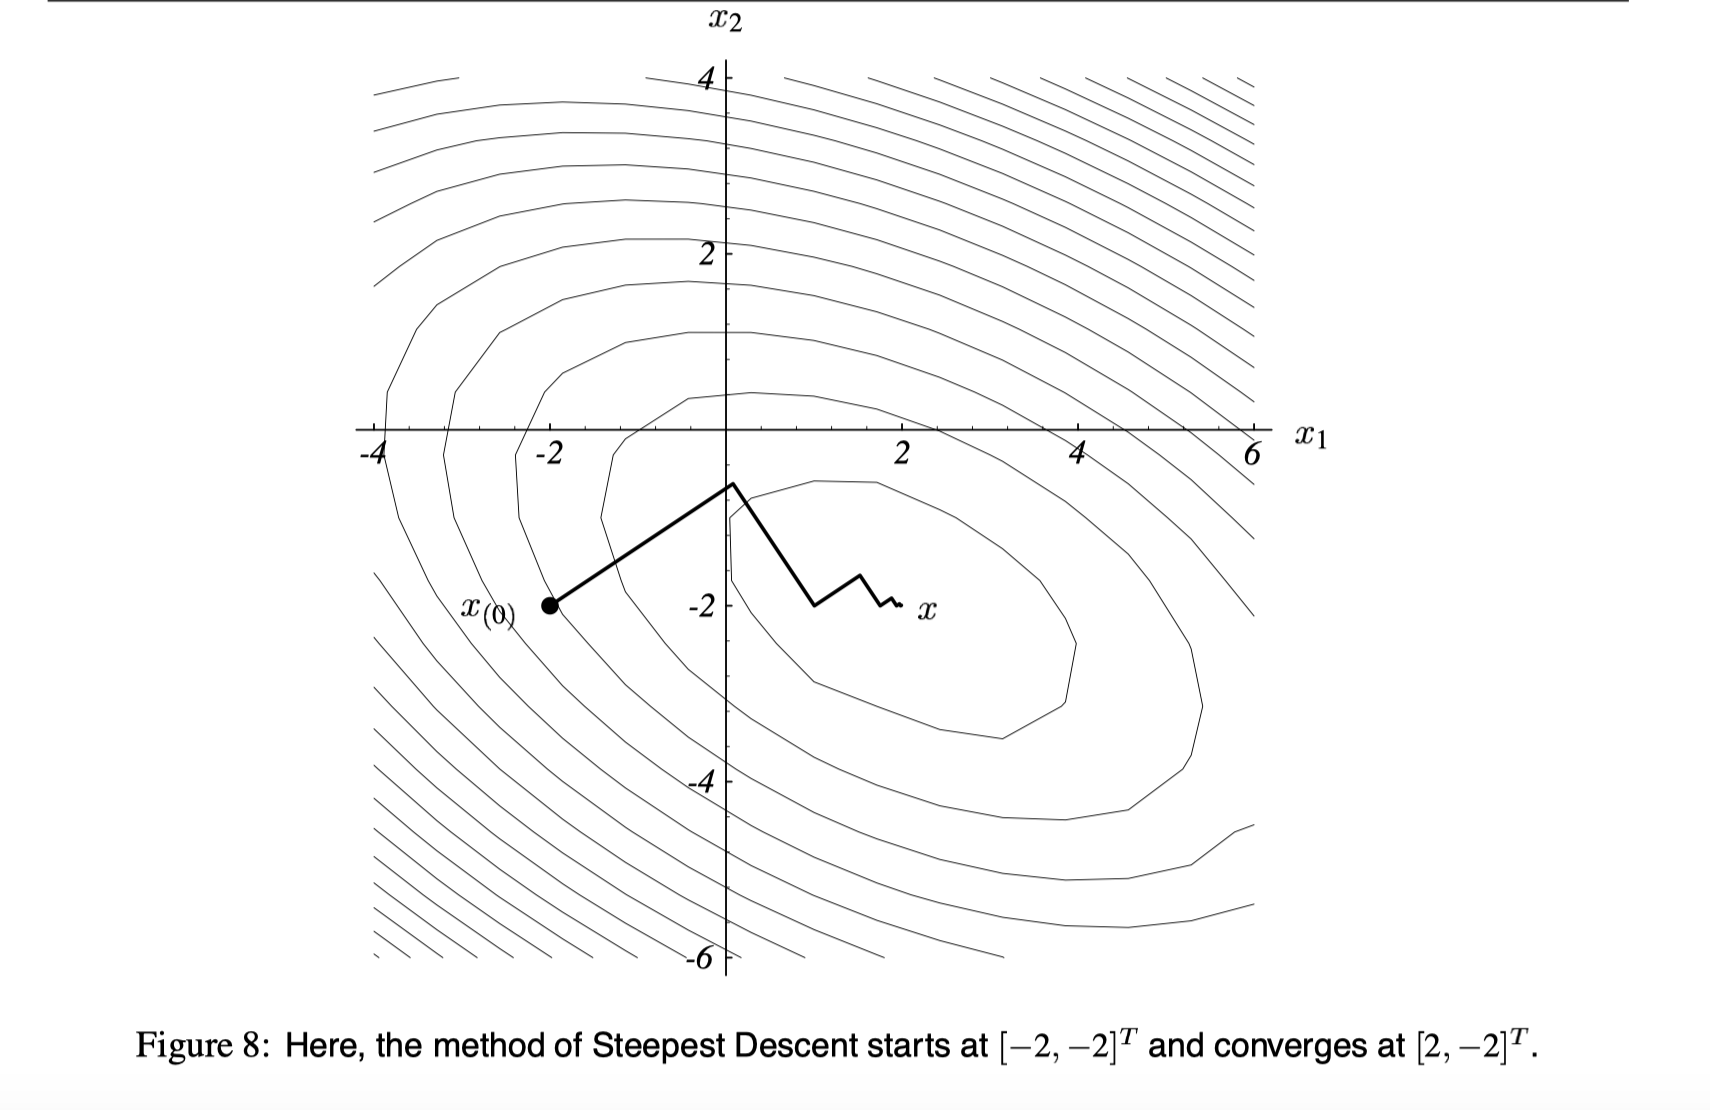
\includegraphics[width=.8\textwidth]{fig/CG_Plot_SD_3.png}
\end{figure}

\section{Jacobi iterations}
\subsection{算法介绍}
使用 Jacobi 迭代法求解 $Ax = b$ 的过程如下:首先将 $A$ 分位两部分:$A = D + E$;其中 $D$ 是 $A$ 的对角元素,其余元素为0;$E$ 是 $A$ 的非对角元素,对角元素为0。然后,按如下步骤求解:
\begin{align*}
Ax &= b \\
(D+E) x &= b \\
Dx &= -Ex + b \\
x &= -D^{-1}Ex + D^{-1}b \\
x &= Bx + z, \qquad B = -D^{-1}E, z = D^{-1}b
\end{align*}

因为 $D$ 是对角线矩阵,所以很容易求逆。同时,观察最后一项:$x = Bx + z$ 可知,该方程的解 $x$ 是其驻点(stationary point),也就是说当 $x_i = x$ 时,有 $x_{i+1} = x$;因此可以按照如下迭代的方法求解 $x$:
$$
x_{i+1} = Bx_i + z
$$

事实上,对 $A$ 进行不同类型的分解,可以得到不同的解法,如 Gauss-Seidel 法,Successive Over-Relaxation(SOR)法等;

\textbf{为了使迭代过程尽快收敛,显然需要 $B$ 有尽量小的谱半径}。

\subsection{收敛性分析}
假定从任意点 $x_0$ 出发,每步迭代都有 $x_{i+1} = Bx_i + z$,将 $x_i$ 分解为 $x$ 和误差 $e_i$ 的和,有:
\begin{align*}
x_{i+1} &= Bx_i + z \\
 	   &= B(x + e_i) + z \\
	   &= Bx + z + Be_i \\
	   &= x + Be_i \\
\therefore e_{i+1} &= Be_i
\end{align*}

所以,如果 $\rho(B) < 1$,那么误差项 $e_i$ 可以收敛至0,也就是说,选择任意初始向量 $x_0$ 都不会影响最终结果。虽然 $x_0$显然会影响迭代步数,但是起决定性因素的还是 $\rho(B)$ 。\textbf{如果 $v_j$ 是$B$ 中具有最大特征值$\lambda_j$ 的特征向量,即 $\rho(B) = \lambda_j$。如果初始误差 $e_0$ 按照 $B$ 的特征向量分解后,包含 $v_j$ 方向的部分,那么这部分收敛至0的速度是最慢的}。

\subsection{Jacobi iterations 算法的缺陷}
一般来说,即使 $A$ 是对称矩阵,$B$ 也未必是对称矩阵;并且,$B$ 可能不存在特征向量;Jacobi iterations 的收敛速度取决于 $rou(B)$,$B$ 又取决于 $A$;然而,即使 $A$ 是正定矩阵,Jacobi 方法也未必能保证收敛。


\subsection{一个具体的例子}
给定矩阵 $A = \begin{bmatrix} 3 & 2 \\ 2 & 6 \end{bmatrix}, b = \begin{bmatrix} 2 \\ -8 \end{bmatrix}$,按照 Jacobi 方法,将 $A$ 进行分解,有:$A = D + E$,其中:
$$
D = \begin{bmatrix} 3 & 0 \\ 0 & 6\end{bmatrix} \qquad E = \begin{bmatrix} 0 & 2 \\ 2 & 0\end{bmatrix}
$$

进而有:
$$
D^{-1} = \begin{bmatrix} 1/3 & 0 \\ 0 & 1/6\end{bmatrix} 
$$
$$
D^{-1} E = \begin{bmatrix} 0 & 2/3 \\ 1/3 & 0\end{bmatrix} \qquad D^{-1} b = \begin{bmatrix} 2/3 \\ -4/3\end{bmatrix} 
$$

所以可以得到如下迭代过程:
\begin{align*}
x_{i+1} &= -D^{-1}Ex + D^{-1}b \\
          &= \begin{bmatrix} 0 & -2/3 \\ -1/3 & 0\end{bmatrix}x_i + \begin{bmatrix} 2/3 \\ -4/3\end{bmatrix}
\end{align*}

$B$ 的特征向量分别为:$v_1 = [\sqrt{2}, 1]^T, v_2 = [-\sqrt{2}, 1]^T$,对应的特征向量分别为:$\lambda_1 = -\sqrt{2}/3, \lambda_2 = \sqrt{2}/3$。从下面的图13(a)可以看出,$B$ 的特征向量与 $A$ 并不重合;图13(b) 表明了 Jacobi 方法的收敛过程,中间每一步的特征向量的变化在图13(c)(d)(e)(f) 中有展示。
\begin{figure}[H]
    \centering
    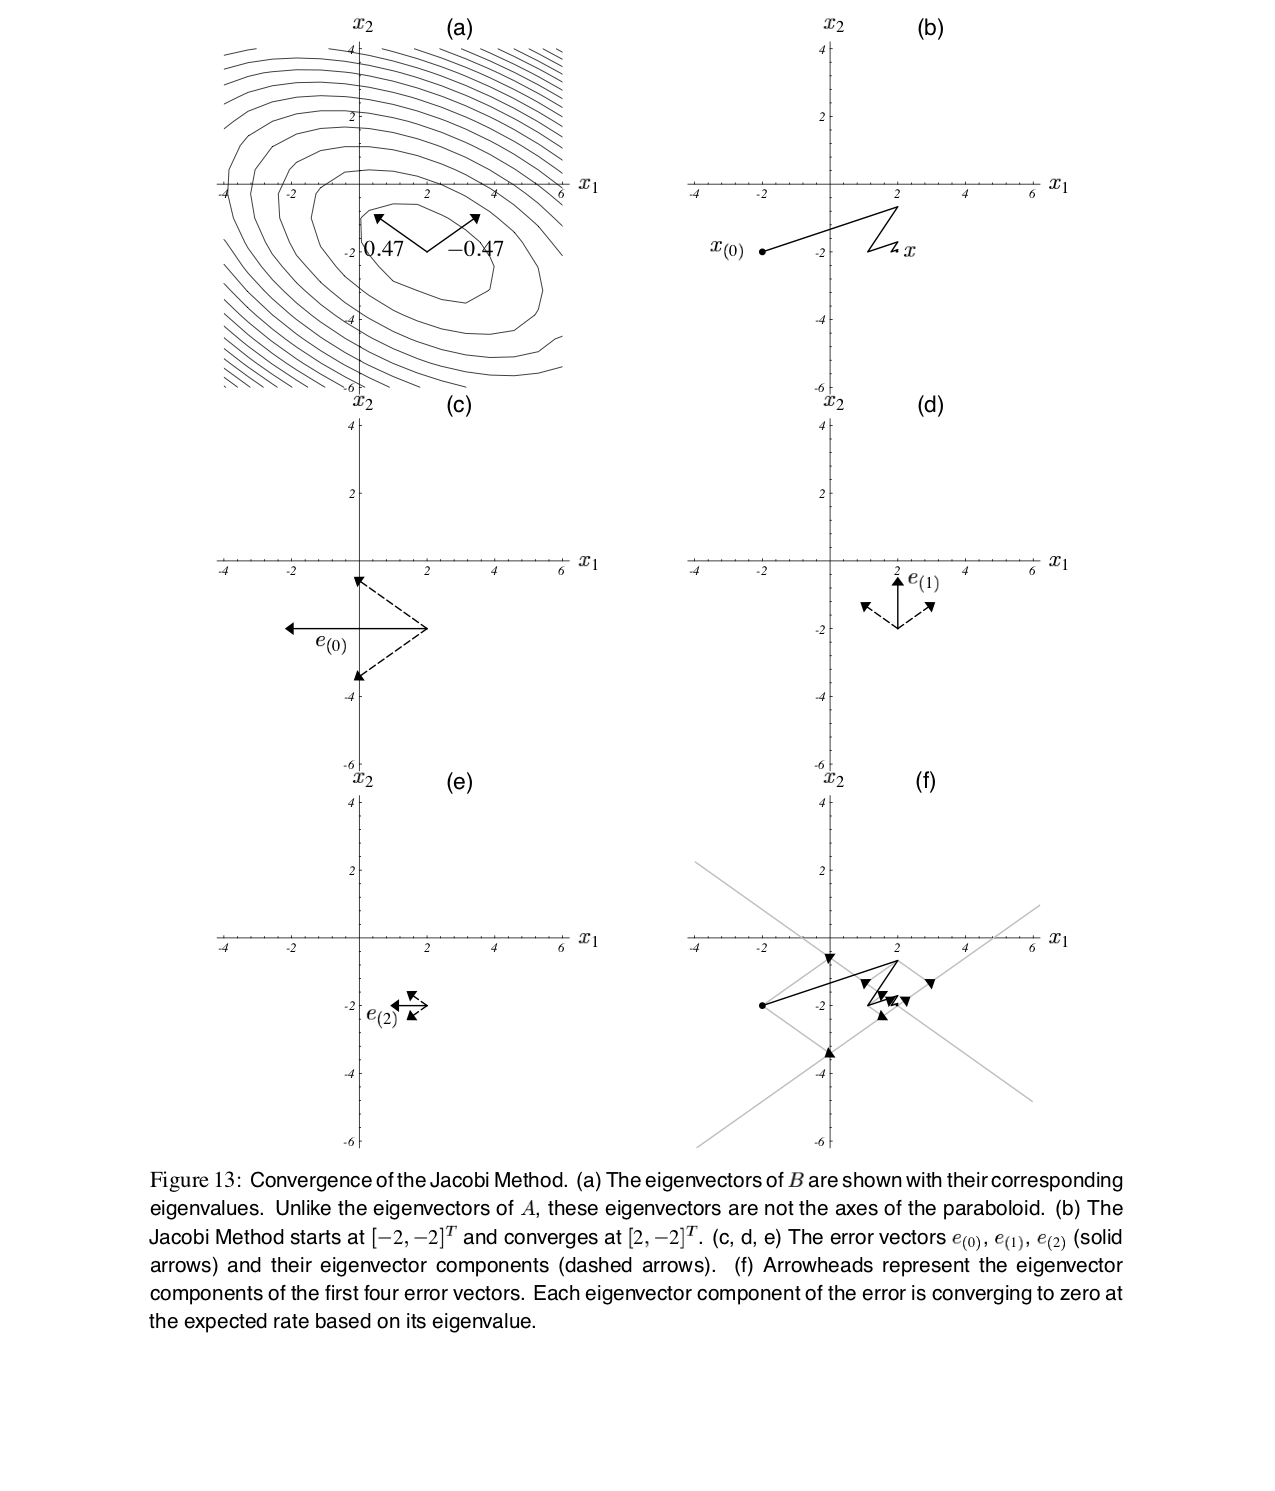
\includegraphics[width=1\textwidth]{fig/CG_Convergence_Jacobi.png}
\end{figure}

\section{最速下降法的收敛性分析}

%\printbibliography
\bibliography{../ref}
\bibliographystyle{IEEEtran}
\end{document}

